\let\negmedspace\undefined
\let\negthickspace\undefined
\documentclass[journal]{IEEEtran}
\usepackage[a5paper, margin=10mm, onecolumn]{geometry}
%\usepackage{lmodern} 
\usepackage{tfrupee} 

\setlength{\headheight}{1cm} 
\setlength{\headsep}{0mm}     

\usepackage{gvv-book}
\usepackage{gvv}
\usepackage{cite}
\usepackage{amsmath,amssymb,amsfonts,amsthm}
\usepackage{algorithmic}
\usepackage{graphicx}
\usepackage{textcomp}
\usepackage{xcolor}
\usepackage{txfonts}
\usepackage{listings}
\usepackage{enumitem}
\usepackage{mathtools}
\usepackage{gensymb}
\usepackage{comment}
\usepackage[breaklinks=true]{hyperref}
\usepackage{tkz-euclide} 
\usepackage{listings}                                        
\def\inputGnumericTable{}                                 
\usepackage[latin1]{inputenc}                                
\usepackage{color}                                            
\usepackage{array}                                            
\usepackage{longtable}                                       
\usepackage{calc}                                             
\usepackage{multirow}                                         
\usepackage{hhline}                                           
\usepackage{ifthen}                                           
\usepackage{lscape}

\begin{document}

\bibliographystyle{IEEEtran}
\vspace{3cm}

\title{4.4.26}
\author{AI25BTECH11030 -Sarvesh Tamgade}
{\let\newpage\relax\maketitle}

\renewcommand{\thefigure}{\theenumi}
\renewcommand{\thetable}{\theenumi}
\setlength{\intextsep}{10pt} 


\numberwithin{equation}{enumi}
\numberwithin{figure}{enumi}
\renewcommand{\thetable}{\theenumi}


\textbf{Question}: Find the equation of the median through vertex \(\vec{A}\) of the triangle \(ABC\), having vertices
\[
\vec{A}(2,5), \quad \vec{B}(-4,9), \quad \vec{C}(-2,-1).
\]
\textbf{Solution:} \\

Using the section formula, the midpoint \(\vec{M}\) of the side \(BC\) is
\[
\vec{M} = \frac{\vec{B} + \vec{C}}{2} = 
\frac{1}{2} \myvec{-4 \\ 9} + 
\frac{1}{2} \myvec{-2 \\ -1} = 
\myvec{-3 \\ 4}.
\tag{0.1}
\]

The median passes through points \(\vec{A} = \myvec{2 \\ 5}\) and \(\vec{M} = \myvec{-3 \\ 4}\).

Let the required line have the equation
\[
\vec{n}^\top \vec{x} = 1,
\tag{0.2}
\]
where
\[
\vec{n} = \myvec{n_1 \\ n_2}
\tag{0.3}
\]
is the column vector (normal vector).

Since both points \(\vec{A}\) and \(\vec{M}\) lie on the median, they satisfy the line equation:
\[
\vec{n}^\top \vec{A} = 1, \quad \vec{n}^\top \vec{M} = 1,
\tag{0.4}
\]
or, explicitly,
\[
\myvec{2 & 5 \\ -3 & 4} \vec{n} = \myvec{1 \\ 1}.
\tag{0.5}
\]

We want to find \(\vec{n}\) satisfying
\[
\myvec{2 & 5 \\ -3 & 4} \vec{n} = \vec{c},
\quad \text{where } \vec{c} = \myvec{1 \\ 1}.
\tag{0.6}
\]

Set up the augmented matrix with right-hand side \(1\):
\[
\myaugvec{2}{
2 & 5 & 1 \\
-3 & 4 & 1
}
\tag{0.7}
\]

Perform row operation \(R_2 \to R_2 + \frac{3}{2} R_1\):
\[
\myaugvec{2}{
2 & 5 & 1 \\
0 & \frac{23}{2} & \frac{5}{2}
}
\tag{0.8}
\]

Perform row operation \(R_1 \to R_1 - \frac{10}{23} R_2\):
\[
\myaugvec{2}{
2 & 0 & -\frac{2}{23} \\
0 & \frac{23}{2} & \frac{5}{2}
}
\tag{0.9}
\]

The final augmented matrix is:
\[
\myaugvec{2}{
2 & 0 & -\frac{2}{23} \\
0 & \frac{23}{2} & \frac{5}{2}
}
\tag{0.10}
\]

Solve the system:
\[
2 n_1 = -\frac{2}{23} \implies n_1 = -\frac{1}{23}
\tag{0.11}
\]

\[
\frac{23}{2} n_2 = \frac{5}{2} \implies n_2 = \frac{5}{23}
\tag{0.12}
\]

\[
\vec{n} = \frac{1}{23} \myvec{-1 \\ 5}
\tag{0.13}
\]

Therefore, equation of required line is:
\[
\boxed{
\myvec{-1 & 5} \vec{x} = 23
}
\]

\begin{figure}[htbp]
    \centering
    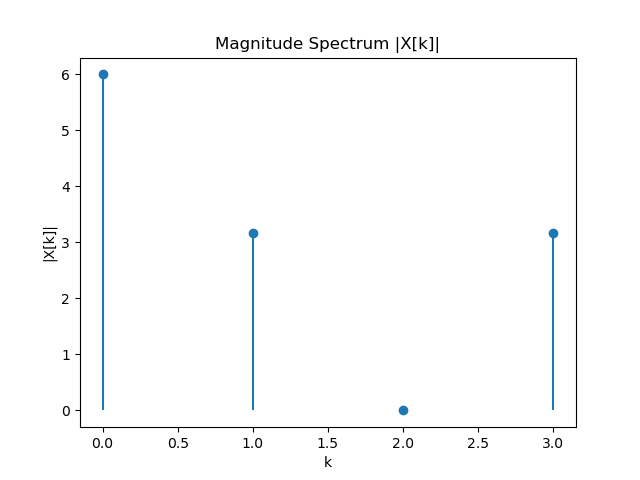
\includegraphics[width=0.65\linewidth]{FIG/fig1.png}
    \caption{Vector Representation}
    \label{fig:FIG/fig1.png}
    \end{figure}

\end{document}  